% -*- LaTeX -*-
% -*- coding: utf-8 -*-
%
% michael a.g. aïvázis
% california institute of technology
% (c) 1998-2010  all rights reserved
%

\section{The hunt for objects}
\label{sec:classes}

The two implementations in \secref{simple:python} and \secref{simple:c} are excellent examples
of a very common occurrence in scientific programming. They are simple and to the point, and
solve the problem as originally stated rather well.  This kind of simplicity has many
advantages: the code is easy to understand, changing it does not require understanding
complicated interactions between unfamiliar pieces of code, and it is likely to have very good
performance characteristics. Unfortunately, even minor attempts at generalization will require
extensive surgery. That's not to say that the time spent in constructing these prototypes is
wasted: it takes foresight that comes with extensive experience to be able to see the general
solution without visiting a few dead ends. As they stand, our two implementations will serve as
benchmarks against which we will judge the next evolutionary steps, and in particular their
performance, so that we can gauge the flexibility trade-off.

There is a variety of approaches one could take to generalize our na\"ive implementation. One
particular paradigm, object oriented programming\supercite{meyer-97}, has proved effective and is
currently very popular. Developers raised on procedural programming, i.e.~the kind of
programming you do in \cc\ or \fortran, typically face a bit of a challenge as they try to shed
inappropriate habits. Those who have managed to climb the learning curve report an increased
awareness of the role of process in software engineering, and overall improvement in the
quality of code they write. However, typical goals such as reuse and flexibility are hard to
attain regardless of the programming paradigm. On one hand, the problem itself has to
co\"operate by belonging to the class of problems that are reducible to fairly orthogonal and
well characterized pieces. On the other, one has to be able to identify these pieces and turn
them into high quality, maintainable code. Much of the time, these form a string of low
probability events that require a significant intellectual investment. Fortunately, the example
at hand is rather well behaved in this regard.

\subsection{Encapsulating the random number generator}
\label{sec:classes:pointcloud}

The first candidate for generalization is the random number generator. We should be able to
choose among many different ones so that we can compare them. In order to take advantage of the
object oriented machinery in languages like python and \cpp, we must identify an appropriate
base class that encapsulates the role the random number generators plays in our integration
algorithm. A moment's reflection should convince you that this role is to provide the cloud of
points that are candidates for evaluating our integrand. The abstract class \class{PointCloud}
will fit this bill very nicely, and its specialization \class{MersenneTwister} will create point
clouds using the Mersenne Twister random number generator we used in \secref{simple:python}. 

Abstract base classes are typically used to anchor class hierarchies. They define the interface
to which derived classes should adhere, but they themselves are not instantiated directly, so
they are not supposed to have any data members and all of their methods should generate
exceptions. We will use \class{PointCloud} to derive classes that hide the implementation
particulars and conform to a standard interface that we will specify.  This idea is that when
we run into another random number generator that we would like to use, the effort necessary to
incorporate it into our program is {\em isolated} to a small subset of the overall code, so
that the likelihood of introducing a bug into the code is minimized.  Ideally, we should need
to do little more than create a new class that derives from \class{PointCloud} and implement
the standard interface using the new generator.

Having identified such a candidate is half the battle; but now a universe of possibilities
opens up. What should its interface be, i.e. what is the list of its class methods? What
arguments should these methods accept? Should there be any data members associated with
instances of this class and its subclasses? A good way to navigate through the possibilities is
to do as little as possible at every step. Rather than trying to anticipate all the possible
uses of \class{PointCloud} and its derivatives, we can focus on endowing it with just enough
interface to solve our problem. We need a sample $X_{N}$ of $N$ random points $x$ that fall
inside a box $B$, so let's create a method \method{point} that takes a suitable representation
of $B$ and returns such a point:
%
\python{
  firstline=9,lastline=24,
  label={lst:classes:pointcloud},
  caption={\srcfile{classes/PointCloud.py}: The abstract base class for representing
    points in the integration region},
}{listings/classes/PointCloud.py}
%
Since \class{PointCloud} is meant to be abstract, we do not attempt to provide a non-trivial
implementation; instead, the method \method{point} raises an exception to remind developers of
derived classes to provide one.

At this stage of the design, we don't have any non-trivial constraints to satisfy. This is both
a blessing and a curse. On one hand, we can pretty much dictate what the class hierarchy will
look like since we are building it from scratch. On the other, there is no structure imposed
from the outside that will help us steer the design is some particular direction. Figuring out
which is a blessing and which a curse is left as an exercise. In these situations, experience
strongly suggests that simplicity and laziness are the right guidelines: defer as many of the
decisions to derived classes as possible, keep the number of methods to a minimum, and make the
interface simple and generic. Unanticipated complexities, such as creating an actual model of
some physical system, or making the code perform at an acceptable level, will force us to
rethink much of the design.

Performance considerations are particularly difficult to anticipate in object oriented
applications. The usual maxims about picking algorithms with low computational complexity and
being careful about the internal structure of loops only capture a fraction of the problem.
Object oriented programs re-shuffle complexity into the interactions of class instances.
Developers are notoriously wrong about what to optimize even in the simplest procedural
routines; it is considerably more difficult to anticipate the performance characteristics of an
object oriented program. The only way to get a clear understanding of which sections of an
application would benefit from further optimization efforts is to use a profiler, a tool
dedicated to analyzing code performance. Despite all the advances in software engineering
technology, it is still very hard to profile a design without an actual implementation. This
deals a rather strong blow to the proponents of formal design practices\supercite{uml} and
makes {\em agile programming}\supercite{agile} a much more attractive methodology for
scientific programming.

One thing is clear: the performance cost of variable accesses and function calls has the
potential to dominate the execution profile of a code in an insidious way. The program may be
too slow, yet the profiler does not uncover any obvious candidates for optimization. This is a
rather unfortunate side effect of object oriented programming, and is one of the reasons that
many scientific programmers stay with the procedural languages or resort to \cpp\ and
templates. Still, much of the code in modern scientific applications deals with the user and
the computational environment; it is these parts that stand to benefit the most from the
complexity management that object oriented techniques bring to the table.

Returning to the problem at hand, we can now derive a class \class{MersenneTwister} that
encapsulates the random number generator from the standard python library that we used in
\secref{simple:python}. We require that \identifier{box} has enough structure so that we can
deduce the dimensionality of the requested point, as well as build the set of transformations
that map from the unit line interval to the corresponding side of the box. The vector diagonal
of the bounding box fits this bill perfectly: we specify that \identifier{box} is to be a pair
of $d$-tuples specifying the coordinates of the point of the box closest to the origin and the
point diagonally across from it. For example, the unit square on the plane might be represented
by \mbox{\tt [[0,0], [1,1]]}, while the unit box in three dimensions would be given by
\mbox{\tt [[0,0,0], [1,1,1]]}.  We only use iterators to access \identifier{box}, so any
iterable container with the structure shown will do.
%
\python{
  firstline=9,lastline=29,
  label={lst:classes:wh},
  caption={\srcfile{classes/MersenneTwister.py}: Encapsulating the standard python generator},
}{listings/classes/MersenneTwister.py}
%
We have unpacked the two corners of the bounding box in the assignment on
\lstlineref{mt:unpack}. On \lstlineref{mt:zip}, we have used \function{zip} to build a tuple of
the co\"ordinate intervals along each axis, over which we iterate in the list comprehension on
\lstlineref{mt:list} in order to provide the arguments to \function{uniform}. The function
\function{uniform} performs the necessary transformations to return a random number between
\identifier{left} and \identifier{right} along each of the axes. The net effect is
a $d$-dimensional random point from the interior of \identifier{box}.

The class \class{PointCloud} and its subclasses should be generally useful to us and are good
candidates for reuse. The interface should be broadened a bit, by adding a means to seed the
random number generator with some initial value, something that most generators support.
Another consideration is that we will be calling this method a large number of times during the
integration, so perhaps we will have to modify the class interface after we evaluate the
performance of this implementation in \secref{classes:driver:draft}.

\TODO{
\item say something about how classes get distributed in files
\item UML diagrams
\item show example of how to encapsulate the GSL random number generator as well
}

\subsection{Representing the region of integration}
\label{sec:classes:region}

The next step in the factorization of the simple implementations in \secref{simple} is to build
a class hierarchy that represents the geometrical properties of the region of integration.
Designing with simplicity in mind would suggest an abstract base class \class{Shape} with a
single method:
%
\python{
  firstline=9,lastline=20,
  label={lst:classes:shape},
  caption={\srcfile{classes/Shape.py}: The base class for the representation of the
    region of integration},
}{listings/classes/Shape.py}
%
from which we derive a class \class{Disk} that represents the interior of a circle.
Completing this representation involves two steps: providing an implementation for
\method{interior} and endowing instances of \class{Disk} with location and size. These two
attributes will be represented as data members of the class that are provided at construction
time, and so they become arguments of the constructor of the class.
%
\python{
  firstline=9,lastline=36,
  label={lst:classes:disk},
  caption={\srcfile{classes/Disk.py}: Representing the interior of a circle},
}{listings/classes/Disk.py}
%
For convenience, the constructor on \lstlineref{disk:constructor} accepts default values for
the radius and the center of the disk. It is best to keep such practices to a minimum because
the implicit passing of information between caller and callee makes the code harder to read and
understand, and they expose users of the class \class{Disk} to the risk that the default values
of the arguments may change in the future. In this case there is a {\em natural} choice for
these values, a unit circle centered at the origin, and so the risk is reduced.

Note that we were careful to avoid injecting the context of our exercise into the design of
\class{Shape} and \class{Disk}. They appear rather generic and their intended use to perform
Monte Carlo integration is not explicit. It is natural to ask a \class{Shape} whether it
contains a given point, regardless of the context for the question. It is not always possible
to avoid this type of pollution, but careful refactoring of the initial design often helps. 

\subsection{The first draft of the object oriented driver}
\label{sec:classes:driver:draft}

We are now ready to put the object oriented solution together and see how it performs. Please
note that we are still assuming that the sampling box is the unit square. Consequently, the
overall normalization necessary to account for the sampling box volume is not shown explicitly.
%
\python{
  firstline=9,lastline=35,
  label=lst:classes:driver,
  caption={\srcfile{classes/gauss.py}: The driver for the objected oriented solution},
}{listings/classes/gauss.py}
%
Before we break open the champagne in celebration of the elegance and simplicity of this
implementation, we have the unfortunate matter of performance to contend with. A look at the
third column of \tabref{classes:simple} should convince you rather quickly that we have a lot
of work still left to do.
\begin{table}
\centering
\[
\begin{array}{r|d{3}d{3}d{3}d{3}d{3}}
% headersep
  & 
  \multicolumn{1}{c}{\cpp} &
  \multicolumn{1}{c}{\mbox{\rm python}} &
  \multicolumn{1}{c}{\mbox{\rm na\"ive OO}} &
  \multicolumn{1}{c}{\mbox{\rm containers}} &
  \multicolumn{1}{c}{\mbox{\rm generators}} \\
% second row
  \multicolumn{1}{c|}{N} &
  \multicolumn{1}{c}{t \mbox{(sec)}} &
  \multicolumn{1}{c}{t \mbox{(sec)}}  &
  \multicolumn{1}{c}{t \mbox{(sec)}}  &
  \multicolumn{1}{c}{t \mbox{(sec)}}  &
  \multicolumn{1}{c}{t \mbox{(sec)}} \\
  \hline \\ [-1.5ex]
% body
  10^{0} &    .002 &    .014 &    .014 &    .014 &    .014 \\
  10^{1} &    .002 &    .014 &    .014 &    .014 &    .014 \\
  10^{2} &    .002 &    .014 &    .014 &    .015 &    .014 \\
  10^{3} &    .002 &    .015 &    .020 &    .019 &    .018 \\
  10^{4} &    .004 &    .027 &    .078 &    .063 &    .053 \\
  10^{5} &    .026 &    .144 &    .625 &    .504 &    .401 \\
  10^{6} &    .230 &   1.265 &   6.242 &   5.925 &   3.780 \\
  10^{7} &   2.277 &  12.624 &  61.583 & 188.318 &  38.242 \\
  10^{8} &  22.749 & 130.430 &         &         &         \\
  10^{9} & 227.735 &         &         &         &         \\
\end{array}        
\]
\caption{Comparison of the cost of the various implementations
  \label{tab:classes:simple}}
\end{table}
%
The object solution is an order of magnitude slower than our previous python implementation,
and almost two orders of magnitude slower than the \cpp\ implementation. 

\TODO{
\item add sentence excusing not going past $10^{8}$
}

\subsection{Improving performance}
\label{sec:classes:improved-performane}

The lackluster performance numbers are not very hard to understand. Taking a closer look at
\lstref{classes:driver} we see that the body of the loop contains two function calls, one to
\method{cloud.point} and another to \method{disk.interior}. Each of these calls is going to get
executed $N$ times and we will have to pay the cost associated with looking up the method name
and calling the associated python functions every time. Furthermore, if you look at the body of
these two functions in \lstref{classes:wh} and \lstref{classes:disk}, you will find quite a bit
of code associated with initializing local variables that have the same value every time these
methods are invoked. That's another cost that we are paying once for each sample point. It
may looks simple enough, but it quickly adds up.

\subsubsection{Containers: trading memory for speed}
\label{sec:classes:containers}

Perhaps we can amortize these costs over the sample set. One approach is to call the random
number generator once and have it build a container with all the points in the sample set. The
representation of the region of integration can act as a {\em filter} by building a container
with the subset of points that fall on its interior. It is important to resist the temptation
to have \class{Shape} just count the points for us so we can avoid the extra container. This
would pollute the design by over-specializing \class{Shape} and would hinder reuse. Further, we
will eventually need to know which points are interior to the \class{Shape} so we can evaluate
our integrand $f$ there.

Turning to the implementation in \lstref{classes:pointcloud:containers}, the class
\class{PointCloud} gets a method \method{points} that expects two arguments: \identifier{n} is
the number of points in our sample, and \identifier{box} is the bounding box representation as
before.
%
\python{
  firstline=9,lastline=25,
  label={lst:classes:pointcloud:containers},
  caption={\srcfile{containers/PointCloud.py}: An improved class for representing the
    evaluation points},
}{listings/containers/PointCloud.py}
%
The new implementation of the subclass \class{MersenneTwister} is shown in
\lstref{classes:mt:containers}. The method \method{points} builds, populates and returns a
container of \identifier{n} random points. The trade off, of course, is that now we must pay
the cost of managing this container. Since $n$ is potentially a large number we must be very
careful inside the \keyword{while} loop. In particular it is important to use \order{1}
operations while building the sample container. Fortunately, \method{append} is very well
behaved in this regard: python lists are implemented in such a way that the interpreter can add
elements at the tail in essentially constant time.
%
\python{
  firstline=9,lastline=33,
  label={lst:classes:mt:containers},
  caption={\srcfile{containers/MersenneTwister.py}: Filling a container with random points},
}{listings/containers/MersenneTwister.py}
%

The abstract class \class{Shape} doesn't require any significant changes. We merely reinterpret
the dummy argument as a container of points and adjust its name accordingly.
%
\python{
  firstline=9,lastline=22,
  label={lst:classes:shape:containers},
  caption={\srcfile{containers/Shape.py}: The base class \class{Shape} requires little
    change},
}{listings/containers/Shape.py}
%
The implementation of \class{Disk}, shown in \lstref{classes:disk:containers}, is only slightly
more complicated than \lstref{classes:disk}. We initialize a container \identifier{keep} and
populate with the interior points.
%
\python{
  firstline=9,lastline=40,
  label={lst:classes:disk:containers},
  caption={\srcfile{containers/Disk.py}: Implementing \class{Disk} as a filter},
}{listings/containers/Disk.py}
%

The driver for the container based solution is shown in \lstref{classes:driver:containers}.
The striking difference with \lstref{classes:driver} is the absence of explicit loops and
counter updates. Instead, we just use the function \function{len} to compute the number of
interior points.
%
\python{
  firstline=9,lastline=33,
  label=lst:classes:driver:containers,
  caption={\srcfile{containers/gauss.py}: The driver for the container based solution},
}{listings/containers/gauss.py}
%

\TODO{
\item compare with the performance in \secref{simple:python} and \secref{classes:driver:draft}
\item talk about the table, and in particular about the $10^{7}$ explosion
}

\subsubsection{Generators: the best of both worlds}
\label{sec:classes:generators}

The container based solution has a certain elegance: the creation of our sample set and its use
are separated into two distinct phases of the computation, the overhead associated with setting
up the calls to the random number generator and the shape instance are amortized over the
sample set, and we can use functions that operate efficiently on lists to perform parts of the
calculation. The major drawback is having to manage the sample container, whose implications
include some overhead in storing and retrieving the contents, and the potential that we run out
of memory for sufficiently large samples.

Fortunately, there is a way to retain the elegance of containers without paying the memory cost
by using {\em generators}, an extremely powerful programming construct borrowed from the
language \identifier{ICON}\supercite{icon}. Hopefully, we will be able to avoid any confusion
between random number generators and the programming construct.

Generators are functions that behave like iterators without necessarily having to manage actual
storage for a container. You can think of them as iterator generators, hence the catchy name.
Explaining what you actually get when you call a generator involves somewhat elaborate
descriptions of python internals; for the purpose of this discussion, you can think of the
result as something that can be used just like a normal iterator. Rather than getting lost in
an abstract description, let's revisit \class{MersenneTwister}. The improvements we will
discuss in this section are focused entirely on the implementation details; the interface as
specified in our abstract classes will remain intact. Hence, we will derive our improved class
from the version of \class{PointCloud} shown in \lstref{classes:pointcloud:containers}. The new
implementation of \class{MersenneTwister} is shown in \lstref{generators:mt}.
%
\python{
  firstline=9,lastline=31,
  label={lst:generators:mt},
  caption={\srcfile{containers/MersenneTwister.py}: The generator based implementation},
}{listings/generators/MersenneTwister.py}
%
Almost everything looks the same as in \lstref{classes:mt:containers}, except for the new
keyword \keyword{yield} on \lstlineref{mt:generators:yield}, and the \keyword{return} without a
value on \lstlineref{mt:generators:return}. Indeed, we unpack the arguments to \method{points}
as we did before, and proceed to loop over the desired sample size, generating ramdom points.
Rather than storing \identifier{p}, we \keyword{yield} it to our caller. This statement
suspends the execution of \method{points} but saves everything that we have done so far,
including the values of all the local variables, such as the loop counter \identifier{n}. The
caller doesn't actually get \identifier{p}, but a type of iterator that executes this code and
returns \identifier{p} when asked for its current value. The magical part is that when the
iterator is asked to advance to advance to the its next item, it will resume evaluating the
method \method{points} at whatever statement follows the \keyword{yield} statement on
\lstlineref{mt:generators:yield} that suspended it. In our case it means that the counter will
get decremented and the loop will execute another iteration until the next time the
\keyword{yield} statement is reached. This process continues until the loop is exhausted, at
which point we run into the \keyword{return} statement on
\lstlineref{mt:generators:return}. According to generator rules, \keyword{return} causes a
\class{StopIteration} exception to be raised, signalling to the caller that we are done
generating values from our virtual container. The \keyword{for} loop quietly handles this
exception and completes the iteration.

If this is making your head hurt, do not worry. It will all make sense pretty soon. Later I
will make your head {\em explode} when we touch on {\em metaclasses}; it seems that some of the
more advanced constructs in python have strange physiological
effects\supercite{guido-metaclasses}.

Let's see what happens to \class{Disk}:
%
\python{
  firstline=9,lastline=39,
  label={lst:generators:disk},
  caption={\srcfile{containers/Disk.py}: Implementing \class{Disk} with a generator},
}{listings/generators/Disk.py}
%
The method \method{contains} still accepts some kind of iterable object \identifier{points} and
goes about the business of deciding whether the contents are interior or not. We set up a loop
over \identifier{points} on \lstlineref{disk:generators:loop}, but rather than storing the
result in \identifier{keep} as we did in \lstref{classes:disk:containers}, we \keyword{yield}
the interior point on\lstlineref{disk:generators:yield}.  When our loops exhausts
\identifier{points} we reach the \keyword{return} statement on
\lstlineref{disk:generators:return}, which raises a \class{StopIteration} exception and
terminates our generator.

All this comes together in the driver shown in \lstref{generators:driver}. The only notable
feature is that we have avoided using the function \function{len} to compute the number of
interior points since it requires an actual container before it can compute sizes. Instead we
use \function{count}, defined in \lstlineref{driver:generators:count}, which updates a counter
as it is looping over the filtered points. See if you can follow how looping over the virtual
contents is driving the generators to produce the associated values without paying the
computational expense to set up the function or manage a container for the intermediate values.
%
\python{
  firstline=10,lastline=43,
  label={lst:generators:driver},
  caption={\srcfile{generators/gauss.py}: The driver for the implementation based on generators},
}{listings/generators/gauss.py}

A glance at \tabref{classes:simple} shows that the generator solution performs rather well. We
are still a bit off the simple python implementation and a whole order of magnitude slower than
\cpp, but such is the price for flexibility.

\subsubsection{Alternative containers}
\label{sec:classes:alternatives}

The container based solution suffers from two drawbacks: the high overhead associated with the
function calls necessary to manage the container, and the large memory footprint of python
containers. Generators enabled us to do away with the temporary storage but do little to
minimize the total number of function calls in the body of the loop. Both of these solutions
are substantially slower than the essentially inlined implementation of \lstref{simple:python}.
Is it possible to improve performance by using better containers than python provides?

At first glance, this looks like a viable strategy. We know the size of the point container
rather early in the program. The points themselves are just pairs of floating point numbers, so
perhaps we can allocate something like a \cc\ array of the right size and hand that to our
random number generator. It's going to be hard to take advantage of the python random number
generator this way, but we can easily access the generators in \package{GSL}, so that's not a big
problem. Once our \cc\ container comes back filled with random points, we should be able to
hand that to a \cc\ routine that will count the interior points. The whole thing can be
orchestrated from python by writing wrappers for the low level routines. We can even recover
the object oriented structure we have been building by using these python wrapped \cc\ routines
as the implementations of the relevant methods of our classes. 

At this point you might be very strongly tempted to write your own array class as a thin
wrapper on top of \cc\ arrays, or even \cpp\ containers. Resist. This thought has occurred to
many a scientific programmer, and the software landscape is littered with such discarded
dysfunctional software. Writing array classes correctly turns out to be much harder than it
appears, mostly due to the fact that containers of real numbers have extremely rich algebraic
structures. You either respect the semantics or you are contributing to the trash heap.

Fortunately, a few of those that didn't get--or didn't pay any attention to--such advice have
tackled this problem and got it right. The package \identifier{numpy}\supercite{numpy} is such an
example. We leave it as an exercise to build and profile a \identifier{numpy}-based solution
that takes advantage of the compactness of representation, speed and convenience of the array
implementation.

How do all these implementations fit together? Do we have to throw away the generators because
we moved the representation to a \identifier{numpy} container? Have we locked ourselves out of
using the python built in random number generator because we cannot feed it a \cc\ array?
Thanks to the fact that interface, rather than type, is what python checks, we can make all
these solutions inter-operate. The generator \identifier{Disk.contains} in
\lstref{generators:disk} does not know or care whether the point container it is
iterating over is real or virtual, a python list or a \identifier{numpy} array. All that
matters is that \identifier{points} is iterable and that each iteration produces a pair of
floats. This lets us keep the object oriented structure and explore various strategies that
trade off between complexity, memory and performance. Better yet, in \secref{components} and
\secref{pyreapp} I will show you how you can let your users assume final responsibility by
postponing making these decisions for as long as possible.

\subsection{Functors}
\label{sec:classes:functors}

The last missing piece of the puzzle is the representation of the integrand. We expect the same
level of flexibility as with every other part of this exercise, so we should be able to
encapsulate functional forms inside appropriate classes, and insert them at the right point in
the integration algorithm. To this end, we create an abstract class \class{Functor} that
specifies the required interface as shown in \lstref{generators:functor}. The only thing
missing to make \class{Functor} a real functor\supercite{c++-idioms} is to connect \method{eval} to
\method{\_\_call\_\_} so that python can recognize subclass instances as callable objects
indistinguishable from normal functions. We'll skip this step since we are not interested in
syntactic sugar at this point of the design; we can always add this later.
%
\python{
  firstline=10,lastline=20,
  label={lst:generators:functor},
  caption={\srcfile{generators/Functor.py}: The abstract base class for functional forms},
}{listings/generators/Functor.py}
%
The method \method{eval} is intended to iterate over the container \identifier{points} and
yield the value of the function at that point. This sounds very sensible at first; there is no
other information about the encapsulated functional form available at the level of the
abstract base class. Then, the part of your brain that has been traumatized by traditional
programming kicks in and raises the question: what about the ``extra'' arguments that functions
usually require? Horror stories of \fortran\ routines with dozens of arguments start flashing
in front of your eyes, and you experience a brief panic attack that this whole object oriented
edifice we have been constructing in these pages is about to collapse. No worries. This is yet
another conceptual success of the object model. The functions in the horror stories are poorly
designed: there are really two kinds of arguments. The first kind is very much the type that
would be presented to a function through \identifier{points}: the point in the domain of the
function where the evaluation is supposed to happen. The other kind is {\em meta-data},
i.e.~information about the functional form itself. For example, consider the expression
\begin{equation}
  g(x; \mu,\sigma) = \frac{1}{\sqrt{2\pi} \sigma} e^{-\frac{(x-\mu)^2}{2\sigma^2}}
\label{eq:gaussian}
\end{equation}
that represents a normal distribution. Languages that do not support objects force you to mix
$x$ with $\mu$ and $\sigma$ in the signature of the function. But they are not really supposed
to be treated on equal footing. Let's suppose that you were asked to plot this expression. It
is almost certain that you would interpret this assignment as follows: fix $\mu$ and $\sigma$
to some nice values, and then sample this function at a few hundred different values of $x$ and
plot the result. You can see that $\mu$ and $\sigma$ do not change as frequently as $x$ does,
which implies that they are not the same kind of data. The implementation of the normal
distribution as a functor shown in \lstref{generators:gaussian} is a much better solution.
%
\python{
  firstline=10,lastline=43,
  label={lst:generators:gaussian},
  caption={\srcfile{generators/Gaussian.py}: Implementation of the normal distribution as a
    functor},
}{listings/generators/Gaussian.py}
%
The two parameters that determine the properties of the distribution become arguments to the
constructor of the functor and so become attributes of the instance that we will use to
represent the integrand. Note that the implementation shown works regardless of the
dimensionality of the domain, thanks to the careful use of functions that operate on
containers. 

In a similar vein, \lstref{generators:constant} shows the implementation of the somewhat
simpler functor \class{Constant} that represents a constant function. Instantiating
\class{Constant} with the parameter \identifier{constant} set to unity will enable us to
reproduce the results of the previous sections.
%
\python{
  firstline=10,lastline=31,
  label={lst:generators:constant},
  caption={\srcfile{generators/Constant.py}: Implementation of constant functions},
}{listings/generators/Constant.py}
%

\subsection{The Monte Carlo integrator}
\label{sec:classes:driver:final}

We are now in a position to put together the final version of the Monte Carlo integrator
script.
%
\python{
  firstline=10,lastline=41,
  label={lst:generators:montecarlo},
  caption={\srcfile{generators/gauss-mc.py}: A Monte Carlo integrator},
}{listings/generators/gauss-mc.py}
%
A comparison between \lstref{generators:montecarlo} and \eqref{mc} shows that there is a nice
correspondence between terms in the equation and objects in the implementation. On
\lstlineref{mc:volume} we compute the volume of the sampling box and us it on
\lstlineref{mc:integral} to scale the average value of the integrand on the points interior to
our region of integration. For this example, we have chosen to perform a non-trivial integral:
a two dimensional version of \eqref{gaussian} is integrated over the unit circle, as shown in
\figref{gaussian}.
%
\begin{figure}
\centering
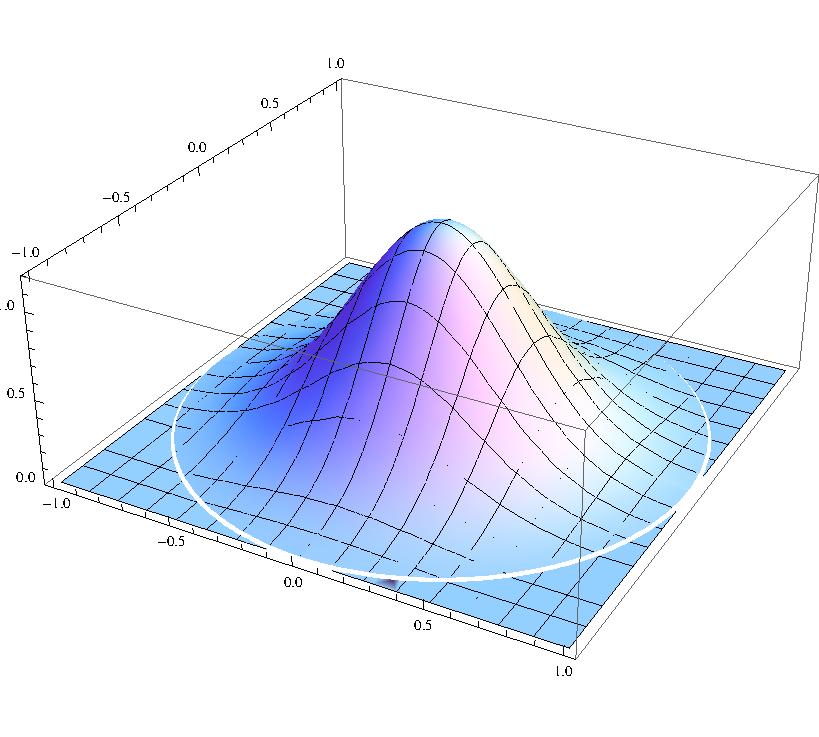
\includegraphics[scale=0.60]{figures/gaussian.pdf}
\caption{The normal distribution of two variables\label{fig:gaussian}}
\end{figure}
%
There are two distinct sections in this script. The top part contains mostly configuration
options while the last few lines are the implementation of the integration algorithm. Computing
an integral over a different region or of a different integrand should be just a matter of
instantiating different objects to hand out to the integration algorithm. At this point, this
involves editing the script and rerunning it; in the next section, I will show you how pyre
makes it possible to have the end user make these choices without touching the source code to
our application script.

% end of file 
